\chapter{Methodology}
The methodology used in this research uses a modification of the classical Grey Wolf Optimization algorithm first introduced by Mirjalili, S., Mirjalili, S., and Lewis, A. in 2014 \cite{Mirjalili2014}. As we will be discussing in this chapter, we have determined that using classical GWO as is does not result in usable solutions for the instance of facility layout problem we are solving. Hence, the necessity for the modification.

In this chapter, we will first discuss about the mathematical model of the problem being solved. Later, we will be delving into the inner workings of the solution representation, the algorithm (including the justification for the modification), and then the technologies that were used in implementing the approach.

\section{Mathematical Model}
The goal of any metaheuristic, like what is being proposed in this paper, is to optimize a certain objective function. As mentioned in the first chapter, in facility layout problems, we minimize the following function:

$$
\text{min} F = \sum_{i=1}^{n}\sum_{j=1}^{n}c_{ij}f_{ij}d_{ij}
$$

For the problem we are solving in this paper, we are optimizing the following equation that is not only a slight modification of the basic mathematical model for FLPs, but also adds penalties to solutions that are infeasible, no matter the degree of infeasiblity.

\begin{align*}
	\text{min }F &= \sum_{i=1}^{\left | B \right |}\sum_{j=i + 1}^{\left | B \right |}c_{ij}d_{ij} \\
	& + \sum_{i=1}^{\left | B \right |}\sum_{j=i + 1}^{\left | B \right |} \left ( P_{B}\frac{A_{0}(i, j)}{\text{min}(w_{i}h_{i}, w_{j}h_{j})} + P_{B} \right ) \cdot \alpha_{0}(i, j) \\
	& + \sum_{i=1}^{\left | B \right |}\left( P_{R}\frac{w_{i}h_{i} - A_{1}(i)}{w_{i}h_{i}} + P_{R} \right) \cdot \alpha_{1}(i)
\end{align*}

where:

\begin{table}[h!]
	\centering
	\begin{tabular}{| l | p{10cm} |}
	\hline
	$x_{i}$  & top-left $x$ coordinate of building $i$ \\
	\hline
	$y_{i}$  & top-left $y$ coordinate of building $i$ \\
	\hline
	$w_{i}$  & width of building $i$ \\
	\hline
	$h_{i}$  & height of building $i$ \\
	\hline
	$R_{x}$  & top-left $x$ coordinate of the bounding region \\
	\hline
	$R_{y}$  & top-left $y$ coordinate of the bounding region \\
	\hline
	$R_{w}$  & width of the bounding region \\
	\hline
	$R_{h}$  & height of the bounding region \\
	\hline
	$c_{ij}$ & flow rate from building $i$ to building $j$ \\
	\hline
	$d_{ij}$ & distance from the center of building $i$ to the
	           center of building $j$ \\
	\hline
	$P_{B}$  & penalty value for building intersection \\
	\hline
	$P_{T}$  & penalty value for any building going out of
	           bounds, even with a portion of a building \\
	\hline
	\end{tabular}
\end{table}

We elected to remove the flow rate from the basic formulation of the model that was discussed earlier in Equation \ref{mm-equation-mhc}. 

\begin{equation}\label{mm-equation-mhc}
	\sum_{i=1}^{\left | B \right |}\sum_{j=i + 1}^{\left | B \right |}c_{ij}d_{ij}
\end{equation}

This is because we can consider flow rate as simply part of the cost. In the original formulation, we were considering it from a material handling cost perspective, which requires having both a cost and flow rate variable. However, in a general problem, we can consider cost to also include the frequency of movement from one facility to another, which is essentially the flow rate. As such, we can merge cost and flow rate into one variable.

The mathematical model allows for infeasible solutions to allow for better solutions in the long run. To follow this specification, the model includes expressions that penalizes solutions that meet any of the following conditions: (1) at least one building is intersecting with another building, and (2) a building, either in whole or in part, is outside the bounding area.

\begin{equation}\label{mm-equation-intersection}
	\sum_{i=1}^{\left | B \right |}\sum_{j=i + 1}^{\left | B \right |} \left ( P_{B}\frac{A_{0}(i, j)}{\text{min}(w_{i}h_{i}, w_{j}h_{j})} + P_{B} \right ) \cdot \alpha_{0}(i, j)
\end{equation}

Equation \ref{mm-equation-intersection} is the expression that applies a penalty to solutions that meet the first condition. Notice that it has the functions $A_{0}(i, j)$ and $\alpha_{0}(i, j)$. They are defined by the following:

\begin{align}
	A_{0}(i, j) &= I_{L}(x_{i}, x_{j}, w_{i}, w_{j})
	               \cdot I_{L}(y_{i}, y_{j}, h_{i}, h_{j}) \\
	I_{L}(x_{1}, x_{2}, l_{1}, l_{2}) &= \text{max}(0, \text{min}(x_{1} + l_{1}, x_{2} + l_{2}) - \text{max}(x_{1}, x_{2})) \\
    \alpha_{0}(i, j) &=
    \left\{\begin{matrix}
    	1 & \text{if } A_{0}(i, j) > 0 \\ 
    	0 & \text{otherwise}
    \end{matrix}\right.
\end{align}

$A_{0}(i, j)$ simply gets the area of intersection of buildings $i$ and $j$. This is achieved by the use of $I_{L}(x_{1}, x_{2}, l_{1}, l_{2})$, which computes the length or width of an intersection of buildings.

In the equation, for every pair of buildings that intersect, we apply a penalty that is the percentage of the area of the smallest building by area that is intersecting with the other building multiplied by the penalty value for building intersection. This will allow for rewarding the algorithm for moving the buildings towards non-intersection. The same penalty value is also added to ensure that the algorithm prioritizes removing intersections over reducing the distance between the centers of the buildings. $\alpha_{0}(i, j)$ ensures that the penalty is only applied to pairs of buildings that intersect with one another.

\begin{equation}\label{mm-equation-oob}
	\sum_{i=1}^{\left | B \right |}\left( P_{R}\frac{w_{i}h_{i} - A_{1}(i)}{w_{i}h_{i}} + P_{R} \right) \cdot \alpha_{1}(i)
\end{equation}

The other part of the mathematical model, Equation \ref{mm-equation-oob}, works in a similar principle as Equation \ref{mm-equation-intersection}. This equation applies a penalty value when the second condition of infeasibility is met. Like in \ref{mm-equation-intersection}, it has specific functions to help compute the penalty. They are defined as:

\begin{align}
	A_{1}(i) &= I_{L}(x_{i}, R_{x}, w_{i}, R_{w})
	\cdot I_{L}(y_{i}, R_{y}, h_{i}, R_{h}) \\
	\alpha_{1}(i) &=
	\left\{
	\begin{matrix}
		0 & \text{if} &
		\begin{aligned}
			R_{x} &\leq x_{i} &\leq R_{x} + R_{w} \\
			R_{x} &\leq x_{i} + w_{i} &\leq R_{x} + R_{w} \\
			R_{y} &\leq y_{i} &\leq R_{y} + R_{h} \\
			R_{y} &\leq y_{i} + h_{i} &\leq R_{y} + R_{h} \\
		\end{aligned} \\		
		1 & \text{otherwise}
	\end{matrix}\right.
\end{align}

$A_{1}(i)$ simply computes the area of intersection of the building and the bounding area. Now, since this only computes the intersection, we must subtract the intersection with the area of the building to get the area of the building that is outside of the bounding area. This is expressed by the numerator of the fractional expression in Equation \ref{mm-equation-oob}. Similar to Equation \ref{mm-equation-intersection}, the equation applies a penalty value that is the percentage of the area of the total building area that is outside the bounding region multiplied and then added by the penalty value. The addition is also to ensure that the algorithm gives more priority to removing out-of-bounds buildings. $\alpha_{1}(i)$ ensures that the penalty is only applied to buildings that are, in part or in whole, out of bounds.

\section{Solution Representation}
The solution is represented using a one-dimensional array of floating numbers. In the array, every group of three consecutive elements are considered to be the x and y positions, and angle, respectively, of one building. While the x and y positions are allowed to be of any value, the angle value is restricted to only $0^{\circ}$ and $90^{\circ}$. A visualization of the solution representation is shown by Figure \ref{solution-repr-viz}.

\begin{figure}
	\begin{center}
		\begin{tabular}{| c | c | c | c | c | c | c |}
			\hline
			$x_{0}$ & $y_{0}$ & $\angle_{0}$ & $\ddots$ & $x_{n - 1}$ & $y_{n - 1}$ & $\angle_{n - 1}$ \\
			\hline
		\end{tabular}
	\end{center}
	\caption{Visualization of the solution representation.}
	\label{solution-repr-viz}
\end{figure}

\section{The Algorithm}
In this paper, we are adapting the Grey Wolf Optimization algorithm into solving our instance of the facility layout problem. There have been no publicly available research that have previously used the metaheuristic in solving FLP, basing from our survey. This increases the significance of this paper. As mentioned earlier, the proposed algorithm requires modifications in order to produce feasible solutions. We will first be discussing the reasons why we require them, before proceeding to detailing the algorithm we are using for this research.

\subsection{The Problem with Classical GWO}
In classical GWO, the following equations are used:

\begin{align}
	\vec{X_{1}^{'}} &= \vec{X_{\alpha}}(t) - \vec{A_{\alpha}} \cdot \vec{D_{\alpha}} \label{gwo-x1-eqn} \\
	\vec{X_{2}^{'}} &= \vec{X_{\beta}}(t) - \vec{A_{\beta}} \cdot \vec{D_{\beta}} \\
	\vec{X_{3}^{'}} &= \vec{X_{\delta}}(t) - \vec{A_{\delta}} \cdot \vec{D_{\delta}} \label{gwo-x3-eqn} \\
	\vec{X}(t + 1)  &= \frac{\vec{X_{1}^{'}} + \vec{X_{2}^{'}} + \vec{X_{3}^{'}}}{3} \label{gwo-xt1-eqn}
\end{align}

where $\vec{X_{\alpha}}$, $\vec{X_{\beta}}$, and $\vec{X_{\delta}}$ represent the $\alpha$, $\beta$, and $\delta$ solutions \cite{Gupta2018}. $\vec{D}$ and $\vec{A}$ are defined as:

\begin{align*}
	\vec{D}        &= \left | \vec{C} \cdot \vec{X_{l}}(t)
	- \vec{X}(t) \right | \\
	\vec{C}        &= 2 \cdot \vec{r_{2}} \\
	\vec{A}        &= 2 \cdot \vec{a} \cdot \vec{r_{1}}
					  - \vec{a}                \\
\end{align*}

The aforementioned equations may be usable as is for other problems. However, as we have discovered through our prior experiments, using these equations results in solutions that are infeasible and where the buildings tend to move to the axes of an origin and the origin itself. One example solution with these characteristics is shown in Figure \ref{bad-solution-unmodified-gwo}, where we have set the origin of the buildings to the center of the bounding region.

\begin{figure}[h!]
	\centering
	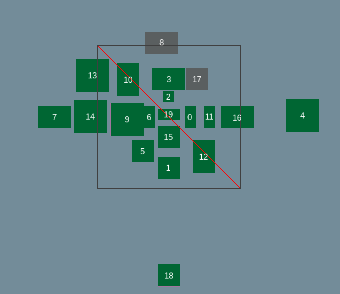
\includegraphics{./images/chap05-methodology/bad-solution-unmodified-gwo.png}
	\caption{Flowchart detailing the algorithm.}
	\label{bad-solution-unmodified-gwo}
\end{figure}

As one may infer, using the equations above will require setting an origin point for the buildings. Not considering the affinity of building towards the axes, having the origin point at the center or in a certain location in the bounding region restricts the possible locations where the buildings can cluster around. This restriction prevents us from exploring the solution subspace where solutions are feasible but where the cluster point is not the origin. This lead us to solutions that are less ideal. Aside from requiring setting the origin point, buildings moving towards the axes also presents another problem. Basing from our experiments, it prevents us from producing feasible solutions.

This behaviour can be attributed primarily to the formula, $\vec{D} = \left | \vec{C} \cdot \vec{X_{p}}(t) - \vec{X}(t) \right |$. To understand why the aforementioned formula contributes to the behaviour we have discussed earlier, we should understand what the formula means. It is helpful to simply consider that only building is being optimized in understanding the problems. Considering only the alpha solution may also provide better understanding as well.

Let us start with $\vec{C} \cdot \vec{X_{l}}(t)$ from $\vec{D} = \left | \vec{C} \cdot \vec{X_{l}}(t) - \vec{X}(t) \right |$. To simplify our explanation, let $K = \vec{C} \cdot \vec{X_{l}}(t)$. The range of each $i$th element in $K$ will be $[0, 2 \cdot \vec{C}_{l,i}]$. Note that the operation is a dot product, but it is actually pairwise multiplication. This means that $K$ simply scales the x and y positions, and angle of the buildings. Figure \ref{gwo-c-effect} shows a visualization of this effect. Despite the figure only showing the effect with a building's position in the first quadrant, the same effect can be observed with other buildings located in other quadrants. Now, considering the entirety of $\vec{D}$, $\vec{D}$ would mean to be the distance between a building $i$ moved to a different point in the region $S$ (see Figure \ref{gwo-c-effect}) in $\vec{X_{l}}$ and a building $i$ in $\vec{X}(t)$. A visualization for this is provided by Figure \ref{gwo-d-effect}.

\begin{figure}[h!]
	\centering
	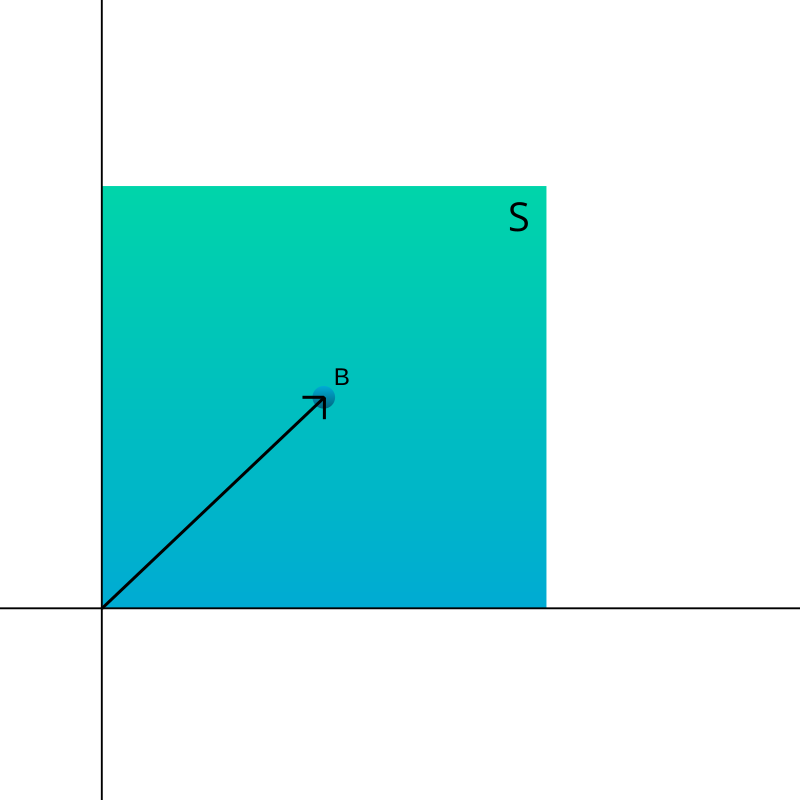
\includegraphics[scale=0.45]{./images/chap05-methodology/gwo-c-effect.png}
	\caption{In $K$, $C$ simply scales the x and y positions and angles of buildings. Assuming that the point $B$ represents the x and y positions of a building, the region $S$ is where $B$ may be repositioned based on the values of $C$.}
	\label{gwo-c-effect}
\end{figure}

\begin{figure}[h!]
	\centering
	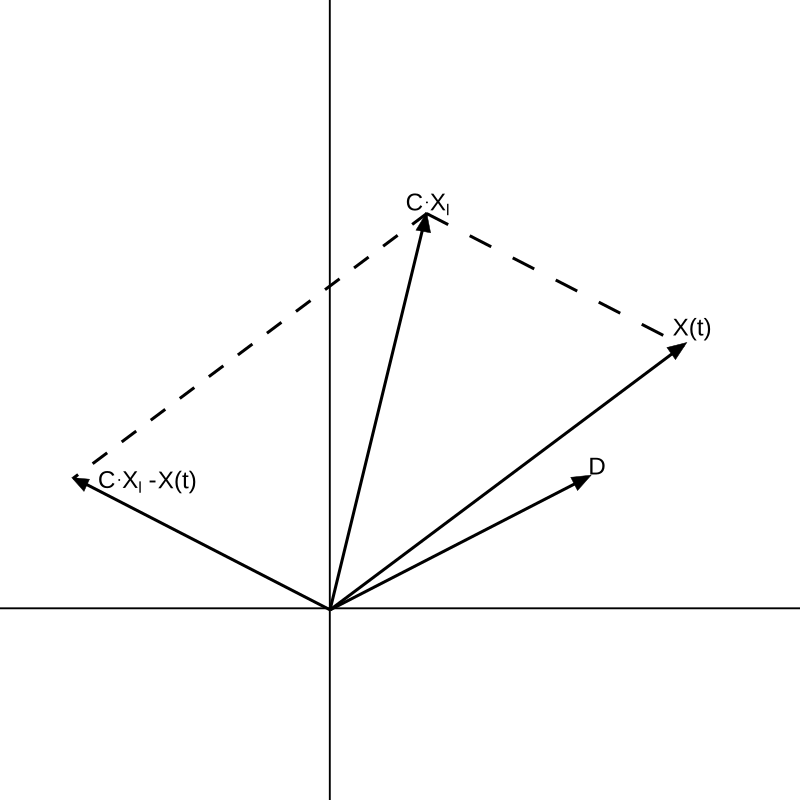
\includegraphics[scale=0.45]{./images/chap05-methodology/gwo-d-effect.png}
	\caption{A visualization of how $D$ is computed and its inherent meaning.}
	\label{gwo-d-effect}
\end{figure}

Let us also take note, $\vec{A} \cdot \vec{D}$. First, we should take note that $\vec{A} = 2 \cdot \vec{a} \cdot \vec{r_{1}} - \vec{a}$. $a$, as mentioned before, linearly decreases over time. Since $a$ decreases linearly over time, $\vec{A}$ will also decrease over time. This behaviour of $\vec{A}$ would mean that in $\vec{A} \cdot \vec{D}$, $\vec{D}$ will eventually decrease as well. Considering equations \ref{gwo-x1-eqn} to \ref{gwo-x3-eqn}, $\vec{A}$ influences the distance of a building from its counterpart in the leading wolves. This would mean that as the number of iterations increase in a run, buildings will eventually follow the placements of the leading wolves.

Let us now return back to $\vec{C} \cdot \vec{X_{l}}(t)$. Over the course of iterations, this equation will make it difficult for a building to change its position. Around 50\% of the time (due to the fact that $\vec{r_{2}}$ is a \textit{uniform} random vector), the value of $\vec{C}$ will be less than $1$. The position of the buildings will be moved towards the axes. Since $\vec{C}$ is a scaling factor, it will be difficult for a building position to move away from an axis. This affects all solutions, and noting that the leading wolves guide the entire population, the movement towards an axis will be propagated towards the entire population, especially with the fact that the $\vec{A}$ reduces the difference between the leading wolves/solutions and the rest of the solutions as the number of iterations increase in a run. Note that the penalty value for intersection prevents them from overlapping with one another. Buildings that are already on a certain axis will find it practically impossible to move in the direction of the perpendicular axis. Buildings that are on the origin itself will practically cease to move at all. Buildings will still be able to change their orientations, however. The reason for this behaviour of being stuck on an axis is due to the nature of axes themselves, where the value in one or both axes is zero, and to the scaling phenomenom caused by $\vec{C}$. Since $K = \vec{C} \cdot \vec{X_{l}}(t)$ and when a building is near or already on an axis, the x, y, or both x and y positions of a building will barely, if at all, move away from the axes it is currently stuck to, when multiplying with $\vec{C}$. Hence, the behaviour we are noticing.

The aforementioned formula makes the classical GWO inadequate for our problem instance. We are unable to produce feasible nor satisfying results. In order for the grey wolf optimization algorithm to be successfully adapted into solving the facility layout problems, we must introduce a few changes into the algorithm. These changes will be discussed in the next subsection.

\subsection{Modified GWO}
\label{methods-section-modified-gwo}
% Draft Note: We should maybe give a name to the modified GWO. Maybe call it "Ballais-Romero GWO variant". HAHAHA.

Mirjalili, S., Mirjalili, S., and Lewis, A. \cite{Mirjalili2014} included a figure similar to Figure \ref{gwo-positioning-update}. It visualizes how a wolf $\omega$ will update its position based on the information provided by the leading wolves.

\begin{figure}[h!]
	\centering
	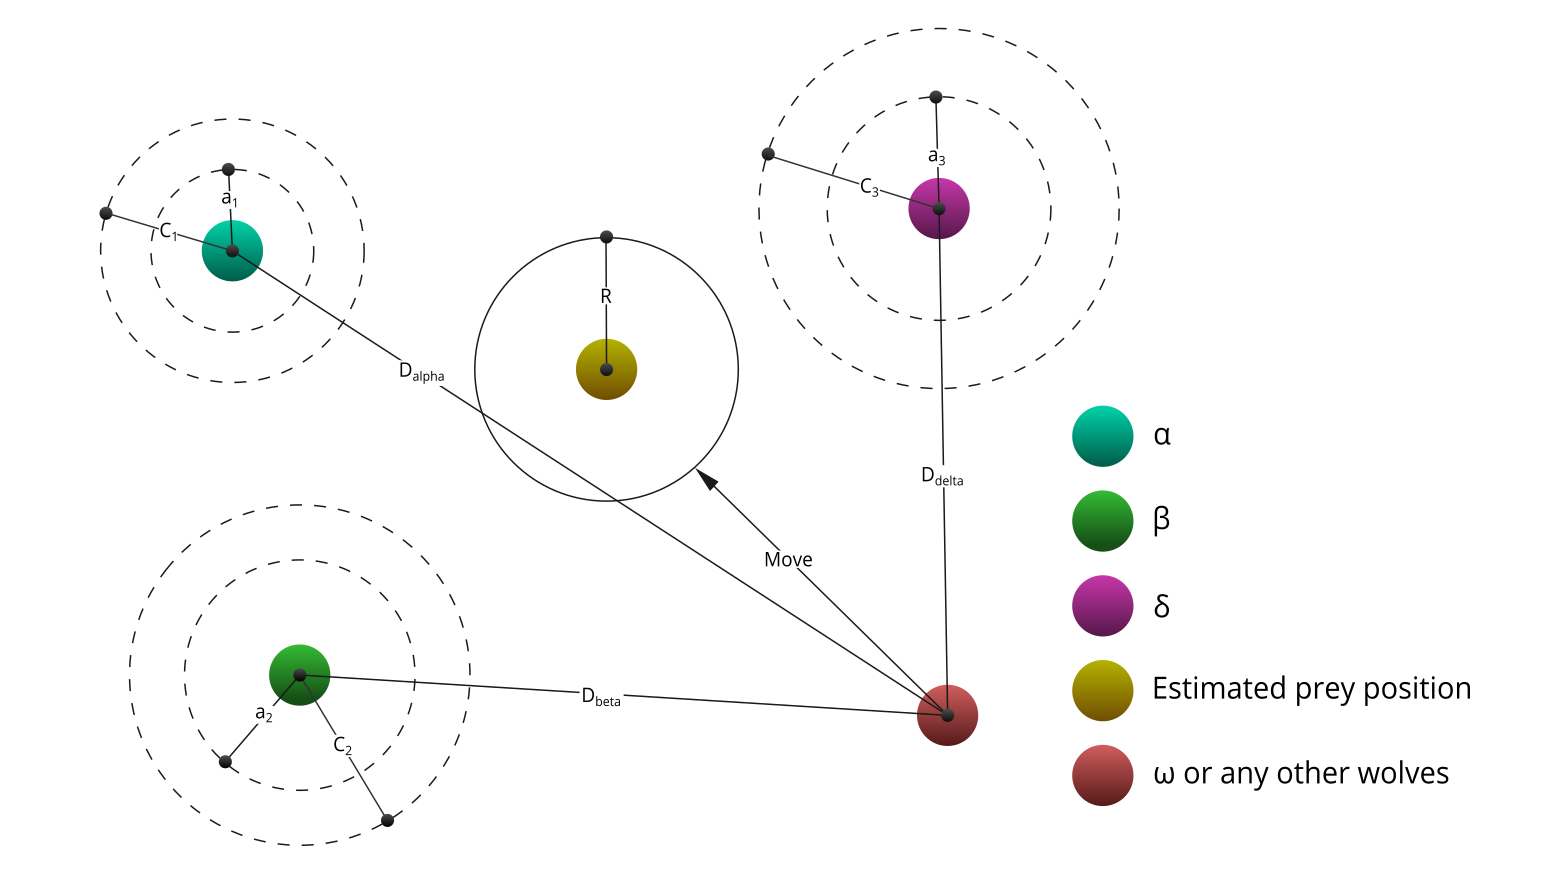
\includegraphics[scale=0.3]{./images/chap05-methodology/gwo-position-updating.png}
	\caption{Visualization of how wolves in GWO update their positions. An $\omega$ wolf will move towards a random point inside the circle of the estimated prey position.}
	\label{gwo-positioning-update}
\end{figure}

Basing from the visualization, notice that the $\vec{C}$ of the leading wolves specify the radius of the circle in which a $\vec{C} \cdot \vec{X_{l}}$ will be located it. The circle does \textbf{not} include an origin point. We have discussed before that performing a pairwise multiplication between $\vec{C}$ and $\vec{X_{l}}$ simply scales the elements $i$ in the vector $\vec{X_{l}}$. This is different from the visualization. To achieve the same effect as the visualization, instead of performing pairwise multiplication, we must utilize vector addition between $\vec{C}$ and $\vec{X_{l}}$. See Figure \ref{vector-addition-visualization} for a visualization of vector addition. This is the first modification we are introducing to classical GWO.

\begin{figure}[h!]
	\centering
	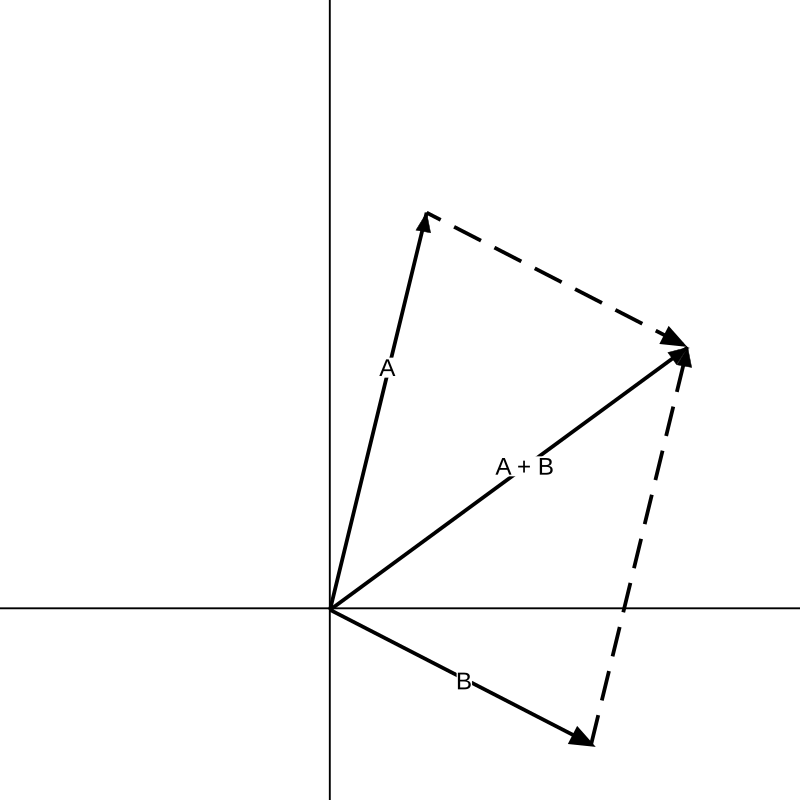
\includegraphics[scale=0.45]{./images/chap05-methodology/vector-addition-visualization.png}
	\caption{Vector addition pushes the point represented by $\vec{A}$ towards the direction of $\vec{B}$ by the magnitude of the same vector.}
	\label{vector-addition-visualization}
\end{figure}

In our modified GWO, $D$ is now defined as:

\begin{align}
	D &= \left | (\vec{C} + \vec{X_{l}}) - \vec{X}(t) \right | \label{modified-gwo-d}
\end{align}

However, this alone is not enough to comply with the aforementioned visualization. Using this will only move the buildings to the right and/or top. In order for us to move the buildings, we must also modify $\vec{C}$ as shown below:

\begin{align}
	C &= c \cdot \vec{r_{3}} \label{modified-gwo-c}
\end{align}

In this equation, $c$ is a real-valued variable, and $r_{3}$ is a random vector in $[-1, 1]$. This modification will now allow us to move a building from any direction and at any magnitude. The magnitude in which the building will be moved is controlled by $c$.

These modifications remove the necessity to specify an origin point in the bounding region, and the behaviour of buildings to move towards the origin or axes. Unfortunately, this alone is not enough to produce feasible results. We have to add two more modifications before we are able to produce good results.

The first additional modification is the building clamping. Each building is restricted to the boundary. If a building is moved towards outside the boundary, it will be pulled back to within the boundary. Building clamping can be mathematically defined as the following. Given a building $B$ in a solution $X(t)$ at iteration $t$ after being updated by Equations \ref{gwo-x1-eqn} to \ref{gwo-xt1-eqn}, \ref{modified-gwo-d}, and \ref{modified-gwo-c}, clamping can be mathematically modeled as:

\begin{align}
	B_{x} &= \text{max}\left (R_{x} + \frac{B_{w}}{2}, \text{min}\left(B_{x}, R_{x} + \left(R_{w} - \frac{B_{w}}{2}\right)\right)\right ) \label{bx-clamp-equation} \\
	B_{y} &= \text{max}\left (R_{y} + \frac{B_{h}}{2}, \text{min}\left(B_{y}, R_{y} + \left(R_{h} - \frac{B_{h}}{2}\right)\right)\right ) \label{by-clamp-equation}
\end{align}

where $B_{x}$ and $B_{y}$ are the $x$ and $y$ positions of the centroid of a building $B$, $B_{w}$ and $B_{h}$ are the width and height from the top left corner of a building $B$, $R_{x}$ and $R_{y}$ are the $x$ and $y$ positions of the top-left corner of the bounding region $R$, and $R_{w}$ and $R_{h}$ are the width and height of the bounding region $R$. Based on our prior experiments, without this clamping, buildings will freely move to points outside the boundary, and, at the end of the run, will produce a bad solution. 

This clamping should \textit{almost} solve the positioning of the buildings and allow us to produce results that are feasible. Since GWO is a continuous metaheuristic, building attributes that must only be one of two values will eventually be a value that is between the two aforementioned values. In our problem, this attribute that is affected is the building orientation. The building orientation may only be $0^{\circ}$ or $90^{\circ}$. It must never be a value between two. To solve this problem, we simply use the orientation of a building $B$ from the $\alpha$, $\beta$, or $\delta$ solutions, which are randomly selected. This idea is based off from the nature of GWO, where the best three solutions lead the search for the local optima. The building orientation of a building $B$ is, therefore, obtained using:

\begin{align}
	B_{o} = \left\{\begin{matrix}
		\alpha_{B_{o}} & \text{if } 0 \leq r < \frac{1}{3} \\ 
		\beta_{B_{o}}  & \text{if } \frac{1}{3} \leq r < \frac{2}{3}  \\ 
		\delta_{B_{o}} & \text{otherwise}
	\end{matrix}\right.
	\label{modified-gwo-bo}
\end{align}

where $B_{o}$ is the current orientation of a building $B$, $\alpha_{B_{o}}$, $\beta_{B_{o}}$, and $\delta_{B_{o}}$ are the orientations of building $B$ in the $\alpha$, $\beta$, and $\delta$ solutions, respectively, and $r$ is a random variable in $[0, 1]$. In our approach, assigning the building orientations is performed before clamping the buildings.

With all these modifications already discussed, we now need to briefly discuss how population initialization performed. The population is initialized by providing each building $B$ a random x and y position values, and random orientation. The orientation is either $0$ or $90$. The x and y positions are clamped as well to ensure that the buildings are inside the bounding region. The positions are clamped using Equations \ref{bx-clamp-equation} and \ref{by-clamp-equation}, respectively. Algorithm \ref{modified-gwo-algorithm-pop-initialization} shows the pseudocode for the population initialization.

\begin{algorithm}[h!]
\caption{Pseudocode for the population initialization.}
\label{modified-gwo-algorithm-pop-initialization}
\begin{algorithmic}[1]
\State Set $\vec{X}$ to be the solution.
\State Set $R_{x}$ to be the x position of the top-left corner of the bounding region $R$.
\State Set $R_{y}$ to be the y position of the top-left corner of bounding region $R$.
\State Set $R_{w}$ to be the width of the bounding region $R$.
\State Set $R_{h}$ to be the height of the bounding region $R$.
\State Set $N$ to be the number of buildings in a population.
\For{i = 0 until $N$}
	\State $\vec{X}_{(i * 3)}$ = $U(R_{x}, R_{x} + R_{w})$
	\State $\vec{X}_{(i * 3) + 1}$ = $U(R_{y}, R_{y} + R_{h})$
	\State $\vec{X}_{(i * 3) + 2}$ = $U({0, 90})$
	
	\State Apply Equation \ref{bx-clamp-equation} to $\vec{X}_{(i * 3)}$.
	\State Apply Equation \ref{by-clamp-equation} to $\vec{X}_{(i * 3) + 1}$.
\EndFor
\end{algorithmic}
\end{algorithm}

All these modifications for the classical GWO have allowed us to successfully adapt GWO to the facility layout problem. Equations \ref{summary-modified-gwo-a} to \ref{summary-modified-gwo-xt1}, and Algorithm \ref{modified-gwo-algorithm} summarises the entire modified GWO. Notice that these modifications are relatively simple, and do not significantly change the characteristics of classical GWO. The simplicity of GWO is still preserved. The next chapters will discuss how our modified version of GWO performs against configurations of unequal-area facility layout ptoblems.

\begin{align}
	\vec{A} &= 2\vec{a} \cdot \vec{r_{1}} - \vec{a} \label{summary-modified-gwo-a} \\
	\vec{C} &= c \cdot \vec{r_{2}} \\
	\vec{D}_{\alpha} &= \left | \left ( \vec{C}_{1} + \vec{X_{\alpha}(t)} \right ) - \vec{X(t)} \right | \label{summary-modified-gwo-DAlpha} \\
	\vec{D}_{\beta} &= \left | \left ( \vec{C}_{2} + \vec{X_{\beta}(t)} \right ) - \vec{X(t)} \right | \\
	\vec{D}_{\delta} &= \left | \left ( \vec{C}_{3} + \vec{X_{\delta}(t)} \right ) - \vec{X(t)} \right | \\
	\vec{X}_{1} &= \vec{X}_{\alpha} - \vec{A}_{1} \cdot \vec{D}_{\alpha} \\
	\vec{X}_{2} &= \vec{X}_{\beta} - \vec{A}_{2} \cdot \vec{D}_{\beta} \\
	\vec{X}_{3} &= \vec{X}_{\delta} - \vec{A}_{3} \cdot \vec{D}_{\delta} \\
	\vec{X}(t + 1) &= \frac{\vec{X}_{1} + \vec{X}_{2} + \vec{X}_{3}}{3} \label{summary-modified-gwo-xt1}
\end{align}

\begin{algorithm}[h!]
\caption{Pseudocode for the proposed modified GWO.}
\label{modified-gwo-algorithm}
\begin{algorithmic}[1]
\State Set $T$ to be the maximum number of iterations.
\State Initialize the grey wolf population $\vec{X}_{i} (i = 1, 2, \ldots, n)$
\State Initialize $c$, and $a = 2$.
\State Calculate the fitness of each wolf.
\State Set $\vec{X}_{\alpha}$ to be the fittest wolf.
\State Set $\vec{X}_{\beta}$ to be the second fittest wolf.
\State Set $\vec{X}_{\delta}$ to be the third fittest wolf.
\While{t $<$ T}
	\For{each wolf $\vec{X}_{i}$}
		\State Initialize $\vec{A}_{1}$, $\vec{A}_{2}$, $\vec{A}_{3}$, $\vec{C}_{1}$, $\vec{C}_{2}$, and $\vec{C}_{3}$.
		\State Update the position of the current wolf $\vec{X}_{i}$ using Equations \ref{summary-modified-gwo-DAlpha} to \ref{summary-modified-gwo-xt1}.
		\State Set the orientation of each building using Equation \ref{modified-gwo-bo}.
		\State Clamp the buildings in $\vec{X}_{i}$ using Equations \ref{bx-clamp-equation} and \ref{by-clamp-equation}.
	\EndFor
	\State Calculate the fitness of each wolf.
	\State Update $\vec{X}_{\alpha}$, $\vec{X}_{\beta}$, and $\vec{X}_{\delta}$.
	\State $a = 2 - \frac{2t}{T}$
	\State $t = t + 1$
\EndWhile \\
\Return $\vec{X}_{\alpha}$
\end{algorithmic}
\end{algorithm}

\section{Implementation Technologies}
Our program was developed using C++17 compiled using the Clang 11 compiler in an elementaryOS Hera environment under release mode with the \texttt{-03} optimized compilation flag turned on. Building was handled by CMake, and package management was handled by Conan. Our implementation is built on top of CoreX, a custom-developed 2D game engine. Using a game engine allowed us to visualize the results and configure experiments in a graphical manner. Using a custom engine over an over-the-shelf engine ensures that the implementation remains light and does not carry unnecessary features that are typically used in commercial game engines. The libraries EASTL, ImGUI, SDL 2, SDL 2 TTF. sdl-gpu, nlohmann JSON, and EnTT were used in developing the engine, with EnTT and ImGUI directly used by our implementation itself.